\section{Diskusjon}

- Hvor i smarttelefonen er sensoren plassert?  \textbf{Fant vel ut at } \newline 
- Bestem aksene (koordinatsystemet) til smarttelefonen. \textbf{se figur \ref{fig:telf_akser} }\newline 
- Hva er oppløsningen til sensoren? \newline
- Er sensoren kalibrert? \newline
- Er målingene stabile? Ser du variasjoner? Er de påvirket av temperatur, lading
osv...? \newline
- Er resultatene reproduserbare etter en reboot/avstengning? \newline
- Kan omgivelsene påvirke målingene?  \newline
- Hva er styrken og retningen til jordens magnetfelt?  \newline
- I hvilken retning er det sanne nord (til nordpolen)? Hvordan bestemme det? \newline
- Kan du detektere lokale variasjoner? Hva kan forårsake disse variasjonene?  \newline
- Avansert: Kan du oppdage variasjoner under døgnet? \newline
- Avansert: Kan nordlys påvirke målingene? \newline

\begin{figure}
    \centering
    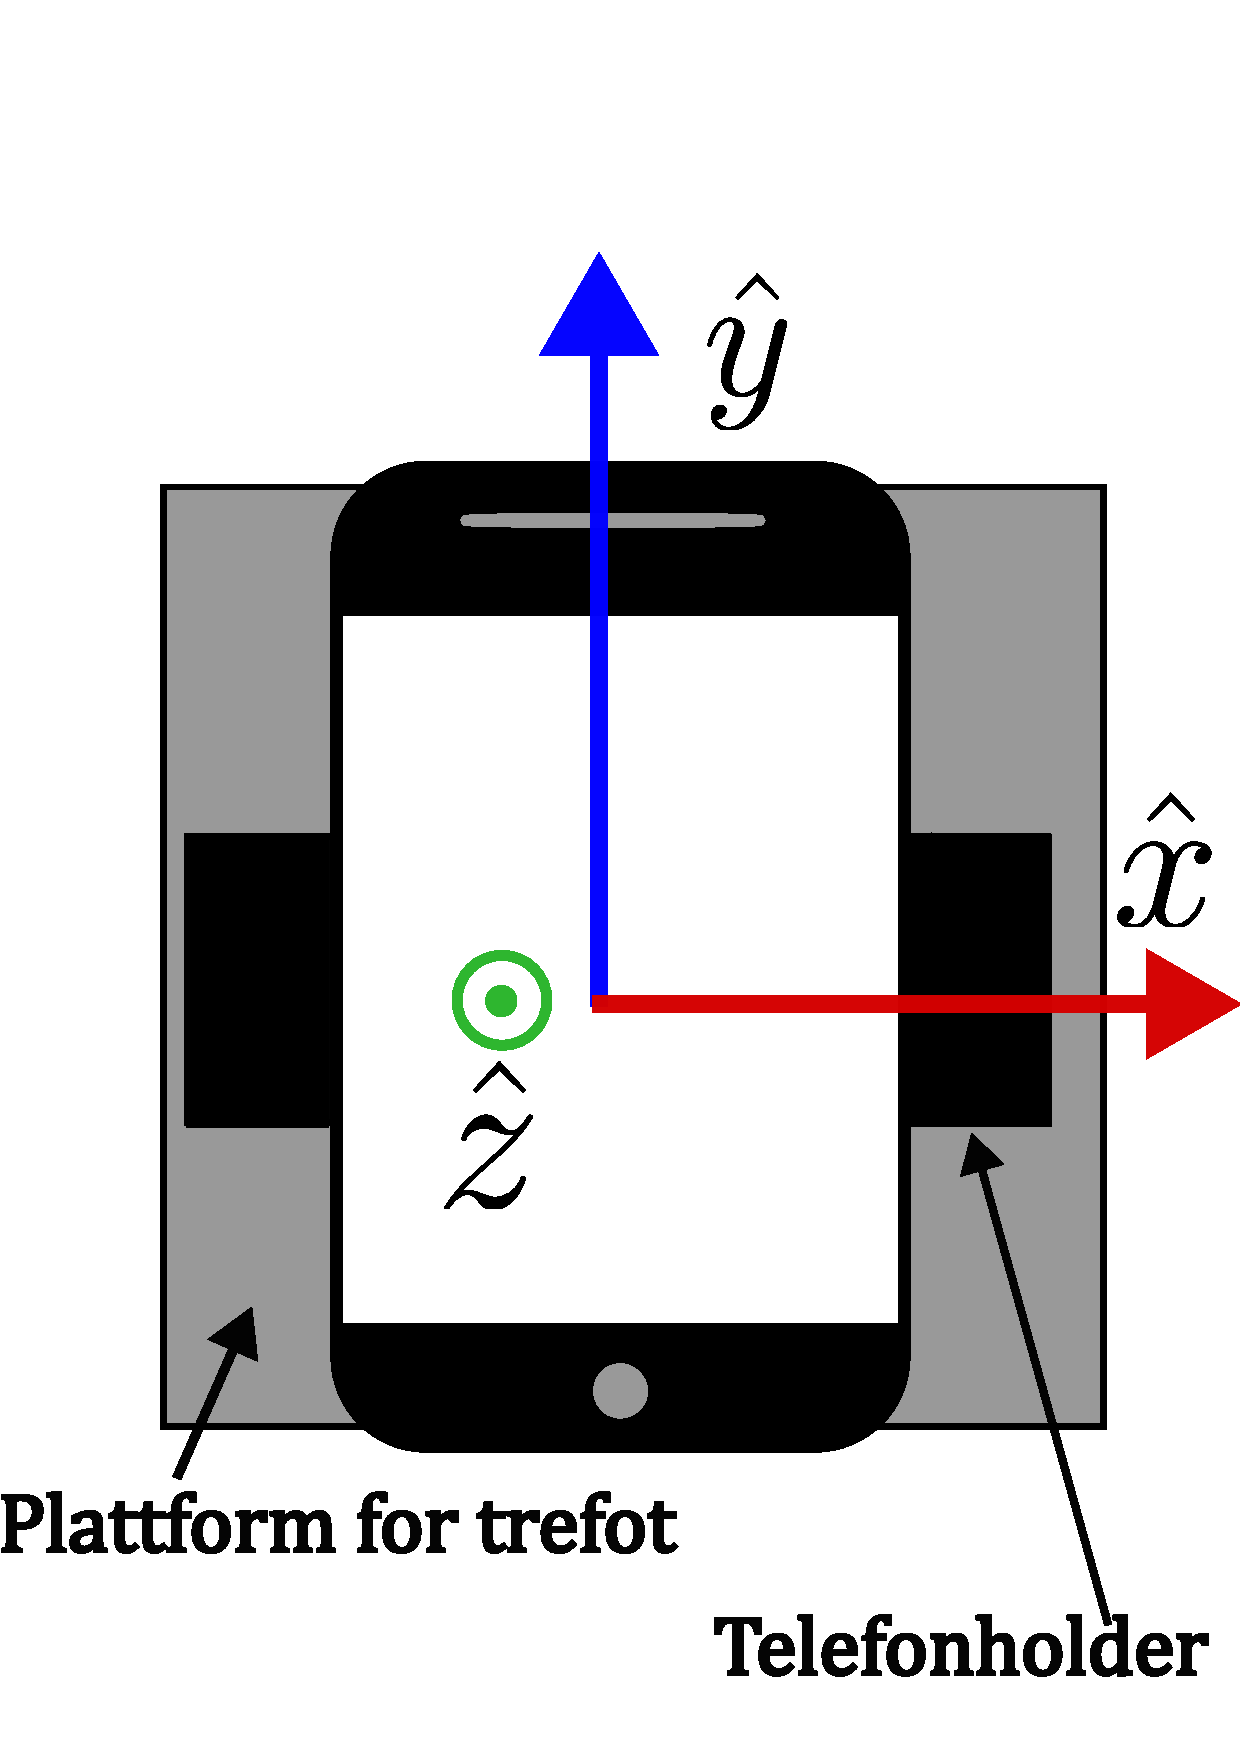
\includegraphics[width=0.65\textwidth]{img/Plattform med telefoni.pdf}
    \caption{\textbf{må kanskje endre på aksene her?} 
        }
    \label{fig:telf_akser}
\end{figure}